\chapter{Urządzenie elektroniczne}

Rozdział zawiera opis części elektronicznej robota z uwzględnieniem mikro kontrolera, czujników inercyjnych oraz interfejsu mocy do silników krokowych. W dalszych podrozdziałach opisane zostały najważniejsze właściwości użytych podzespołów sterownika oraz sposób ich integracji. 

\section{Sterownik}

Sterownik robota oparty jest o płytkę ewaluacyjną STM32F3 Discovery z mikroprocesorem STM32F303VCT6. Rozwiązanie to udostępnia znaczną moc obliczeniową i pozwala na zastosowanie bardziej zaawansowanych algorytmów sterujących. Najważniejsze cechy modułu STM32F3 Discovery: 

	\begin{tabular}{  l   p{3cm} |}
	-Rdzeń: Cortex M4F \\
	-Taktowanie 72 MHz  \\
	-256 kB Flash \\
	-48kB RAM \\
	-3- osiowy, cyfrowy żyroskop L3GD20 \\
	-3- osiowy, cyfrowy akcelerometr z magnetometrem LSM303DLHC \\
	-10 diod LED  \\
	-Dwa przyciski 		 \\	
\end{tabular}  




Wykorzystanie elementów umieszczonych na płytce ewaluacyjnej pozwala zredukować wykorzystanie dodatkowych podzespołów o niezbędne w projekcie czujniki inercyjne oraz ułatwiające proces projektowy diody i przyciski. Schemat demonstrujący sposób komunikacji podzespołów sterownika znajduje się na rysunku \ref{schemat}



\begin{figure}[h]
	\centering
	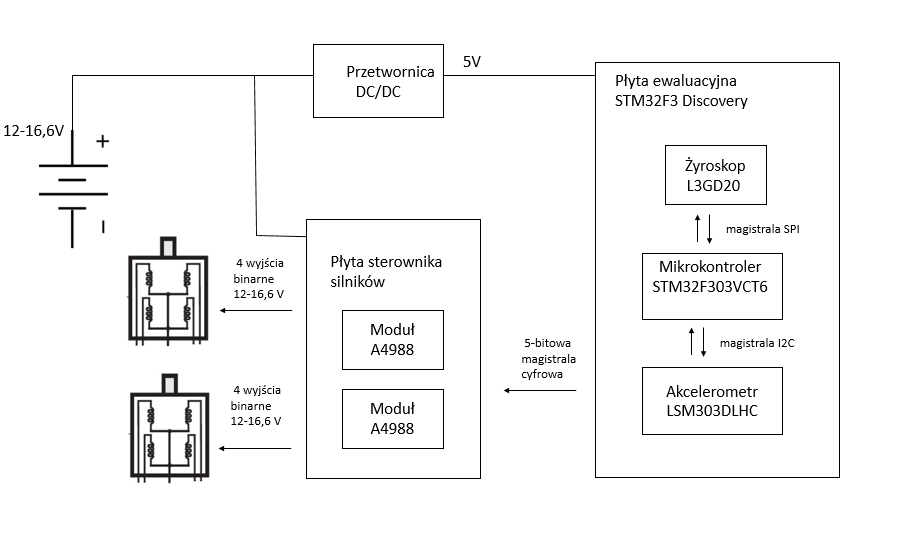
\includegraphics[scale=0.6]{schemat_sterownika.png}
	\caption{ Schemat steroniwka. Grafika własna}
	\label{schemat}
\end{figure}


\section{Żyroskop}

Wykorzystane żyroskop to zawarty na płytce ewaluacyjnej układ L3GD20. Jest to trójosiowy żyroskop cyfrowy. Jego kluczowe właściwości to:

\begin{tabular}{  l   p{3cm} |}
	 -Trzy dostępne skale pomiarowe (250/500/2000 dps) \\
	 -Interfejs komunikacyjny $I^2C$ lub $SPI$\\
	-16 bitowa rozdzielczość pomiarów \\
\end{tabular}  

W projekcie komunikacja z czujnikiem przebiega przy użyciu protokołu SPI. Wykorzystywana skala pomiarowa to: 500 dps.


\section{Akcelerometr}
Kolejnym wykorzystanym elementem płytki ewaluacyjnej jest trójosiowy akcelerometr z magnetometrem LSM303DLHC. 

\begin{tabular}{  l   p{3cm} |}
	- Interfejs komunikacyjny: I2Cm\\
	-Akcelerometr, zakres: $\pm$ 2 g, $\pm$ 4 g, $\pm$ 8 g oraz $\pm$ 16 g\\
	-Magnetometr, zakres:  od $\pm$ 1,3 do $\pm$ 8,1 gauss\\
	-16 bitowa rozdzielczość pomiarów \\
\end{tabular}  


Sensor został skonfigurowany na zagres $\pm$2g. Mangetometr nie został wykorzystany ze względu na znaczne zakłócenia wskazań poprzez niewielką odległość od silników .


\section{Sterownik silników krokowych}

Do kontroli silników krokowych wykorzystany został sterownik stworzony na potrzeby pracy inżynierskiej. Jest on oparty o 2 układy A4988, każdy z nich pozwala sterować pojedyńczym silnikiem za pomocą dwóch wyprowadzeń cyfrowych.Zbocze narastające na drugim powoduje wykonanie kroku w kierunku ustawionym przez stan drugiego wyprowadzenia. Sterowniki pozwalają na sterowanie mikrokrowoe w trybie 1/2, 1/4, 1/8 i 1/16 kroku. W projekcie silniki zostały skonfigurowanę na pracę w trybie 1/8 kroku, pojedyńczy krok w tym trybie obraca wał o 0.225 stopnia.  Ustawienie to dostarcza wystarczającą precyzję sterowania. Użycie pracy w trybie 1/16 kroku zmniejszyłoby moment oborotowy silników a dalsze zwięszkanie precyzji sterowania nie jest konieczne.


\section{Zasilanie}

Robot jest zasilany przy pomocy 4 ogniw litowo-jonowych połączonych szeregowo. Są to niezależne ogniwa 18650 o napięciu znamionowym 3.7V i pojemności około 2200mAh. Napięcie całego pakietu waha się od 16.8V przy pełnym naładowaniu do 12V w stanie rozładowania akumulatorów. Elektronika zasilana jest przy pomocy regulowanej przetwornicy impulsowej dostarczającej napięcie 5V. Sterownik silników zasilany jest bezpośrednio z akumulatorów w związku z czym ich zachowanie zależne jest od stopnia rozładowania.


